
%
% Prepared for Phys. Rev. X
% Topics: Nuclear Physics & Statistical Physics 
%

\documentclass[10pt,aps,prc,twocolumn]{revtex4-1}

\usepackage{tabularx} 
\usepackage{graphicx} 
\usepackage{hyperref}  
\usepackage{amssymb}  
\usepackage{amsmath}  
\usepackage[]{units}

\bibliographystyle{apsrev4-1}

\begin{document}
\title{Bias-Variance Tradeoff and Model Selection for Proton Radius Extractions}
% a.k.a. How I Learned to Stop Worrying and Love the Bias

\author{Douglas Weadon Higinbotham}
\affiliation{Jefferson Lab, Newport News, VA 23606}
\author{Randall Evan McClellan}
\affiliation{Jefferson Lab, Newport News, VA 23606}
\author{Xuefei Yan}
\affiliation{Duke University, Durham, NC 27708}
%\affiliation{Jo\v{z}ef Stefan Institute, SI-1000 Ljubljana, Slovenia}
\author{Miha Mihovilovi\v{c}}
\author{Simon \v{S}irca}
\affiliation{Faculty of Mathematics and Physics, University of Ljubljana,
SI-1000 Ljubljana, Slovenia}
\affiliation{Jo\v{z}ef Stefan Institute, SI-1000 Ljubljana, Slovenia}

\begin{abstract}
Intuitively, a scientist might assume that a more complex model will necessarily yield a more 
accurate description of experimental data.   Herein, we disprove this notion in the context of extracting 
the proton charge radius from simulated charge form factor data.  We will show that, for a given set of data, 
a biased parsimonious model can in fact have greater predictive power than a less-biased, more-complex model.  
Perhaps more surprising,
we will also show that in certain cases a parsimonious model can even be a better predictive model 
than the true generating function.   While illustrated for the case of radius extraction of electron scattering data,
this result provides an important example of the fact that a scientist cannot achieve a better result by
over-parameterization or over-elaboration.   With these ideas in mind, we take a careful step-by-step look at the
latest low $Q^2$, high precision electron scattering data and using Bayesian Information Critian extract a proton 
radius of 0.842(8)~fm.
\end{abstract}

\maketitle

\section{Introduction}

High-precision Lamb shift experiments on muonic atoms have determined the proton radius to 
be 0.84087(39)~fm~\cite{Pohl:2010zza,Antognini:1900ns}.   This result is in stark contrast to the current
CODATA recommended value of 0.875~fm~\cite{Mohr:2015ccw} which comes from an average of atomic 
Lamb shift and electron scattering results.    This difference has become known in the literature as
the proton radius puzzle~\cite{Pohl:2013yb}.

While initial efforts to understand this puzzle focused on the details of the muonic experiment, attention has
now turned to re-examining the atomic and electron scattering results.   In fact, the first of the
new generation of published atomic Lamb shift measurements is in statistical agreement with the muonic 
result~\cite{Beyer79} though preliminary findings from another group agree with the classic atomic 
results~\cite{fleurbaey:tel-01633631}.

For the electron scattering data, the proton's charge radius, $r_p$, is extracted from
cross section data by determining the slope of the electric form factor, $G_E$, in the
limit of four-moment transfer, $Q^2$, approaching zero: 
\begin{equation}
\label{eq:radius}
  r_p \equiv %\sqrt{ \langle r^2 \rangle} =
    \left( -6  \left. \frac{dG_E(Q^2)}{dQ^2}
    \right|_{Q^{2}=0} \right)^{1/2} \>.
\end{equation}
Of course, electron scattering cannot reach the exact $Q^2 = 0$ limit; thus,
an extrapolation is required to extract the charge radius from the experimental data.

Many methods have been proposed to make this extrapolation,
ranging from parsimonious fits of low $Q^2$ data~\cite{Rosenfelder:1999cd,Griffioen:2015hta,Horbatsch:2015qda,Higinbotham:2015rja},
to extremely complex fits with tens of free parameters~\cite{Bernauer:2010wm,Bernauer:2013tpr,Lee:2015jqa,Graczyk:2014lba,Lorenz:2014vha}.
In additional to statistical modeling, there are of course 
theory inspired extractions of the radius~\cite{Belushkin:2006qa,Horbatsch:2016ilr}.   These also tend to favor the 
muonic radius, leading to a conclusion that either there is a problem with the parsimonious low $Q^2$ fits or physics beyond
what is included in current calculations~\cite{Carlson:2015jba,Liu:2016qwd}.
Inspired by the illustration in Krauth~{\it{et al.}}~\cite{Krauth:2017ijq}, we made a collection
of the proton radius extractions in Fig.~\ref{collection}.    In general, the low $Q^2$ parsimonious fits
and the ChPT inspired modeling tend to agree with the $\mu H$ result, while the more complex fitting
tends to agree with the CODATA value.   The detail that is effecting all the results is how the normalization
of the experimental data is handled.

\begin{figure}
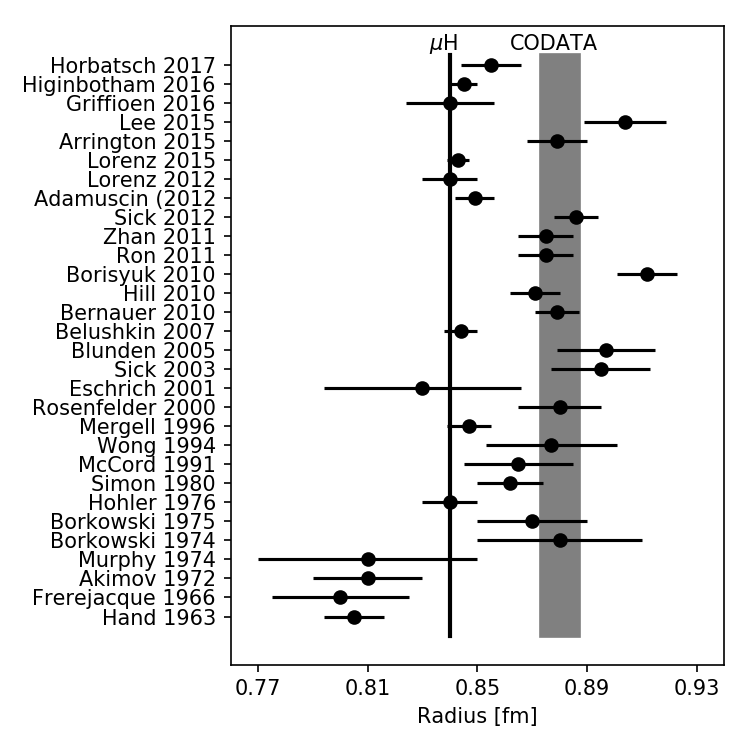
\includegraphics[width=\columnwidth]{Figure/ScatteringResults.png}
\caption{Collection of radii extracted from electron scattering data:  
Horbatsch~2016~{\cite{Horbatsch:2016ilr}}
Higinbotham~2016~{\cite{Higinbotham:2015rja}},
Griffioen~2016~{\cite{Griffioen:2015hta}},
Lee~2015~{\cite{Lee:2015jqa}},
Arrington~2015~{\cite{Arrington:2015ria}},
Lorenz~2015~{\cite{Lorenz:2014yda,Lorenz:2014vha}},
Lorenz~2012~{\cite{Lorenz:2012tm}},
Adamuscin~2012~{\cite{Adamuscin:2012zz}},
Sick~2012~{\cite{Sick:2012zz}},
Zhan~2011~{\cite{Zhan:2011ji}},
Ron~2011~{\cite{Ron:2011rd}},
Borisyuk~2010~{\cite{Borisyuk:2009mg}},
Hill~2010~{\cite{Hill:2010yb}},
Bernauer~2010~{\cite{Bernauer:2010wm}},
Belushkin~2006~{\cite{Belushkin:2006qa}},
Blunden~2005~{\cite{Blunden:2005jv}},
Sick~2003~{\cite{Sick:2003gm}},
Eschrich~2001~\cite{GoughEschrich:2001ji},
Rosenfelder~2000~{\cite{Rosenfelder:1999cd}},
Mergell~1996~{\cite{Mergell:1995bf}},
Wong~1994~\cite{Wong:1994sy},
McCord~1991~\cite{McCord:1991sd},
Simon~1980~\cite{Simon:1980hu},
Hohler~1976~\cite{Hohler:1976ax},
Borkowski~1975~\cite{Borkowski:1975},
Borkowski~1974~\cite{Borkowski:1974tm,Borkowski:1974mb}
Akimov~1972~\cite{Akimov:1972nu},
Murphy~1974~\cite{Murphy:1974zz}, and
Frerejacque~1965~\cite{Frerejacque:1965ic}, and
Hand~1963~\cite{Hand:1963zz}.}
\label{collection}
\end{figure}

A general criticism of the parsimonious extractions of the proton radius is the presence of bias~\cite{Sick:2017aor,Sick:2018fzn},
with an implication that bias needs to be completely avoided in order to successfully extract the true radius from the data.
The use of bias to reject parsimonious proton radius extraction methods dates back to the classic Monte Carlo 
study of Borkowski~{\it{et al.}}~\cite{Borkowski:1975} where linear extrapolates were flatly rejected in favor of quadratic
extrapolations.  Herein we will show that when using a Monte Carlo study to test a model's ability
to extract the proton radius, one needs to consider not only bias but also the variance and illustrate how 
the best predictive model to use will depend on the range, quantity and precision of the data.
This will illustrate how a biased parsimonious model can in fact have a higher predictive 
validity than an unbiased less parsimonious model.   In addition, we will then apply these ideas to model selection with real
data, where instead of millions of Monte Carlo results, we get but a single realization of the possible outcomes.  


\section{Bias}

In the English language bias is often used as a pejorative term, while in the context of regression, it is simply
an offset from the ideal distribution.   It is important to note, that since it is part of a distribution it
is not a property of a single realization but determined by repeated sampling.    In the context of the proton 
radius extractions, bias was nicely illustrated by Borkowski~{\it{et al.}}~\cite{Borkowski:1975} and we will
illustrate their procedure in the following.

Randomly generate sets of form factor pseudo data 
from $\unit[0.1]{fm^{-2}}$ to 0.4, 0.8, 1.2,
and $\unit[1.6]{fm^{-2}}$ 
in steps of $\unit[0.05]{fm^{-2}}$ 
using the standard dipole function:
\begin{equation}
\label{sd}
G\mathrm{_D}(Q^2) = ( 1 + Q^2/(\unit[18.27]{fm^{-2}}))^{-2},
\end{equation}
where the cutoff parameter of 18.27~fm$^{-2}$ corresponds to a radius of 0.8097~fm.
To mimic real data, the data points were randomly smeared with a normal distribution
with a sigma of 0.5\%.  
Next, perform fits on the resulting sets of pseudo data with linear and quadratic functions:
\begin{align}
f_{\mathrm{linear}}(Q^2) &  = a_0 + a_1 Q^2, \label{Eq:linear} \\
f_{\mathrm{quadratic}}(Q^2) & = a_0 + a_1 Q^2 + a_2 Q^4. \label{Eq:quadratic}
\end{align}
These functions are written so that they are linear in the fit coefficients.  
This allows the $\chi^2$ minimization to be performed exactly
and also allowing the normalization to float.   Since it is known that
G$_E$(0) = 1, it is common practice to factor out the normalization term, $a_0$, and 
then the slope of G$_E$(0) is given by $a_1/a_0$ and can be used in Eq.~\ref{eq:radius} 
to determine the radius.

This procedure was done with $10^6$ sets of pseudo data to 
precisely determine the mean of the extracted 
radii for these two models.   Since we used standard dipole as the input function, one would expect an unbiased 
function to return a radius of 0.8097~fm.
Table~\ref{ztable} reproduces the original result~\cite{Borkowski:1975} and
an example code is provided in the supplemental material of our paper.  
As the table clearly shows, the mean of linear fits shows a clear bias. 
Accordingly, the authors of the original work concluded that the linear models 
should always be rejected in favor of the lower-bias quadratic function.
They then proceeded to extract the proton charge radius from real data using a five parameter 
fit: a quadratic charge form factor and three floating normalizations.

\begin{table}
\caption{The mean $a_0$ and radius from doing $10^6$ Monte Carlo simulations
for each interval in $Q^2$
where Eq.~\ref{sd} was used to generate pseudo data in $\unit[0.05]{fm^{-2}}$ steps
with each data point smeared by a randomly generated, normally distributed point-to-point 
uncertainty of 0.5\%.
The results clearly indicate that the linear fits are biased.   The input
radius was \unit[0.8113]{fm} (an $a_1/a_0$ term of $\unit[0.1097]{fm^{-1}}$) and $a_0 = 1$.}
\begin{tabular}{c|cc|cc} \hline
interval       & \multicolumn{2}{c|}{linear fit} & \multicolumn{2}{c}{quadratic fit}  \\
fm$^{-2}$      & $a_0$      & Radius [fm]          & $a_0$    & Radius [fm] \\ \hline
 0.1 -- 0.4 & 1.000& 0.79& 1.000& 0.81 \\
 0.1 -- 0.8 & 0.999& 0.78& 1.000& 0.81 \\
 0.1 -- 1.2 & 0.997& 0.77& 1.000& 0.81 \\
 0.1 -- 1.6 & 0.996& 0.76& 1.000& 0.81 \\ \hline
\end{tabular}
\label{ztable}
\end{table}


\section{Variance}

While it is true that the linear fit exhibits a bias, it is not the only parameter that needs
to be considered when selecting which model to use for extrapolating the radius.
In particular, one should also consider the variance.
Table~\ref{fulltable} shows a more complete picture of the simulation results 
where the width of the fit, sigma, is 
shown along with the bias.   This is graphically represented in Fig.~1 where it becomes clear that 
for the low $Q^2$ intervals, the linear fits clearly provide results that are closer to
the input radius than the quadratic fits, while for the larger intervals the quadratic becomes
the more appropriate function.
Thus this simple example problem becomes a nearly textbook illustration of the trade-off between 
variance and bias with the linear fit having a relatively high bias with a low variance, while the 
quadratic fits have a low bias and high variance.

\begin{table*}
\caption{An expanded version of Table~\ref{ztable} where instead of just showing the mean offset of the 
fit results, the bias, we also indicate the width of the fit results, sigma.   Also shown is the
root mean square error, RMSE, which can be used to quantify the best function for a given interval.}
\begin{tabular}{cc|cccccc|cccccc} \hline
Data   & Interval     & \multicolumn{6}{c|}{linear fit}                       & \multicolumn{6}{c}{quadratic fit}                    \\ 
Points & fm$^{-2}$ &   $a_0$  & Radius [fm]&  $a_1/a_0$ &  Bias  & Sigma &  RMSE  &   $a_0$  & Radius [fm]& $a_1/a_0$  &  Bias  & Sigma &  RMSE \\  \hline
7      & 0.1 -- 0.4 & 0.9995& 0.7948& $-0.1053$& $-0.0044$& 0.0184& 0.0189 & 1.0000& 0.8063& $-0.1084$& $-0.0013$& 0.1094& 0.1094\\
15     & 0.1 -- 0.8 & 0.9987& 0.7828& $-0.1021$& $-0.0076$& 0.0057& 0.0095 & 1.0000& 0.8096& $-0.1092$& $-0.0005$& 0.0281& 0.0281\\
22     & 0.1 -- 1.2 & 0.9975& 0.7712& $-0.0991$& $-0.0106$& 0.0030& 0.0110 & 0.9999& 0.8089& $-0.1090$& $-0.0007$& 0.0138& 0.0138\\
31     & 0.1 -- 1.6 & 0.9959& 0.7600& $-0.0963$& $-0.0134$& 0.0019& 0.0136 & 0.9998& 0.8075& $-0.1087$& $-0.0010$& 0.0085& 0.0085\\ \hline
\end{tabular}
\label{fulltable}
\end{table*}

\begin{figure}[htbp]
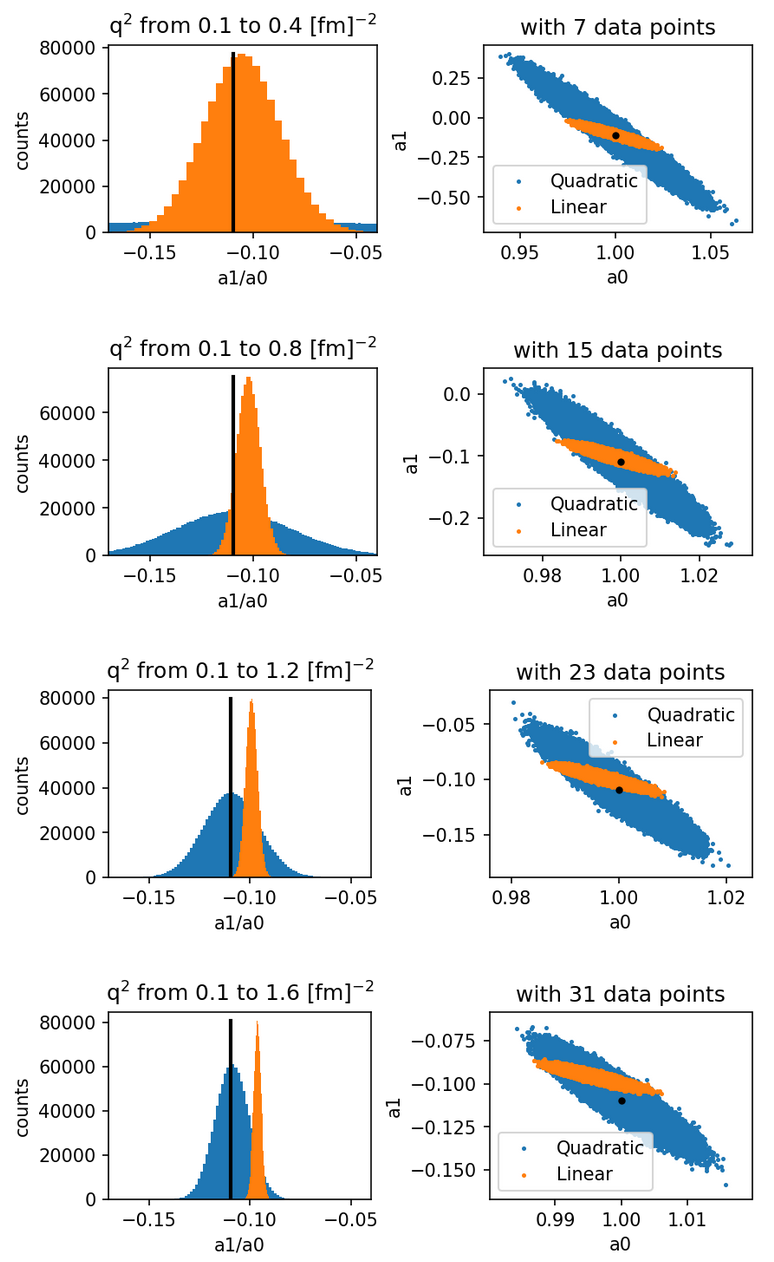
\includegraphics[width=\columnwidth]{Figure/zresult.png}
\caption{A graphic representation of the Monte Carlo results showing how the linear fits tend to have a relatively
high bias though a low variance, while the quadratic fits tend to have a relatively low bias but a large variance.}
\end{figure}

\begin{table*}
\caption{Same as Table~\ref{fulltable}, but now with equal number of data points of each range.}
\begin{tabular}{cc|cccccc|cccccc} \hline
Data   & Interval  & \multicolumn{6}{c|}{linear fit}                       & \multicolumn{6}{c}{quadratic fit}                    \\ 
Points & fm$^{-2}$ &   $a_0$  & Radius [fm]&  $a_1/a_0$ &  Bias  & Sigma &  RMSE  &   $a_0$  & Radius [fm]& $a_1/a_0$  &  Bias  & Sigma &  RMSE \\  \hline
31& 0.1 -- 0.4 & 0.9995& 0.7951& $-0.1054$& $-0.0043$& 0.0098& 0.0107 & 1.0000& 0.8090& $-0.1091$& $-0.0006$& 0.0629& 0.0629 \\
31& 0.1 -- 0.8 & 0.9987& 0.7829& $-0.1021$& $-0.0076$& 0.0041& 0.0086 & 1.0000& 0.8099& $-0.1093$& $-0.0004$& 0.0208& 0.0208  \\
31& 0.1 -- 1.2 & 0.9974& 0.7712& $-0.0991$& $-0.0106$& 0.0026& 0.0109 & 0.9999& 0.8089& $-0.1091$& $-0.0006$& 0.0121& 0.0121  \\
31& 0.1 -- 1.6 & 0.9959& 0.7600& $-0.0963$& $-0.0134$& 0.0019& 0.0136 & 0.9998& 0.8076& $-0.1087$& $-0.0010$& 0.0085& 0.0085  \\  \hline
\end{tabular}
\label{equaldatatable}
\end{table*}

\section{Goldilocks Dilemma}

For any given set of statistical models, the goal is to find the optimal balance between bias and variance.   
As was noted by George Box, all models are wrong, thus the goal is to find the most appropriate one. 
In general, this can be written as
\begin{equation}
\frac{d {\mathrm{Bias}^2 }}{ d {\mathrm{Complexity}}} = \frac{- d {\mathrm{Variance}} }{ d {\mathrm{Complexity}}},
\end{equation}
as illustrated in Fig.~\ref{biasvariance}.
Thus to quantify the goodness of the fits, we use Root Mean Square Error (RMSE),
\begin{equation}
{\mathrm{RMSE}} = \sqrt{ {\mathrm{bias}}^2 + {\mathrm{Sigma}}^2} = \sqrt{{\mathrm{Bias}}^2 + {\mathrm{Variance}}}.
\end{equation}

Going back to Table~\ref{fulltable} and checking the Root Mean Square Error, RMSE, one can now quantify 
that for this example the 0.1 -- 0.8~fm$^{-2}$ interval is optimal for the linear model while the 0.1 -- 1.6~fm$^{-2}$ 
interval is optimal for the quadratic model. 
This is in contrast to the conclusion one draws when one only considers bias as presented in Table~\ref{ztable},
though consistent with the observation that the optimal specific form of the parameterization 
may depend on the $Q^2$ region being fit~\cite{Alberico:2008sz}.
\begin{figure}
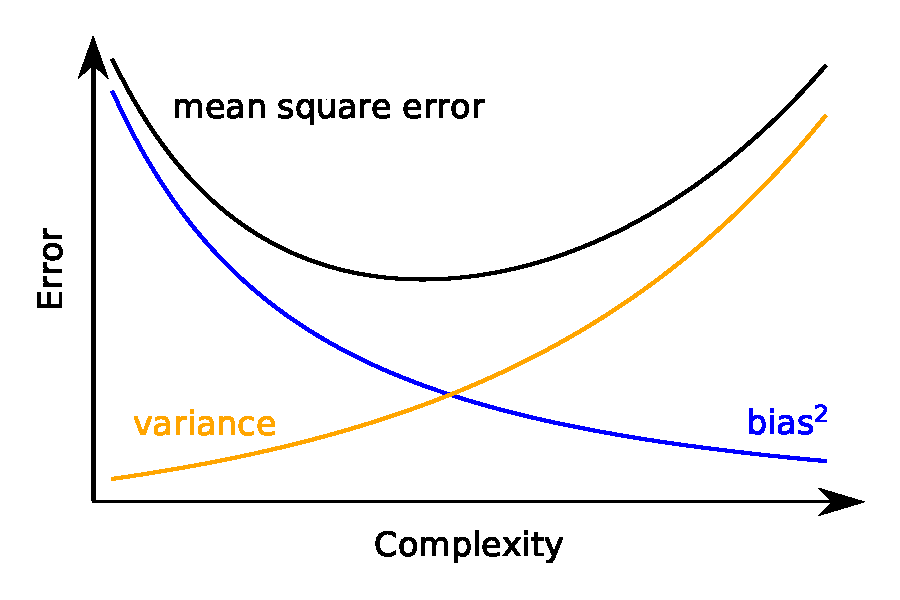
\includegraphics[width=\columnwidth]{Figure/biasvariance-clean.pdf}
\caption{An illustration of the trade-off between bias and variance when selecting a statistical model.   Simple models
will have low variance but high bias (under-fitting) while complex models will have low bias but high variance (over-fitting).   
It is this trade-off that one seeks to balance.   While with repeated  Monte Carlo simulations it is trivial to find the optimal
predictive model for a given set of data, in the real world the true model is typically unknown; one only gets to perform
a very limited number of experiments and thus one relies on using real data and statistical methods for 
model selection~\cite{Hastie:2009}.}
\label{biasvariance}
\end{figure}

It is interesting to repeat the Monte Carlo simulation for equal number of data points within each range
especially since for elastic scattering cross sections are significantly higher at lower values of $Q^2$
and thus it is easy to obtain more low $Q^2$ data.
This is shown in Table~\ref{equaldatatable} and now the picture is even grayer as the RMSE of the linear 
fit is nearly equal to the quadratic, thus, assuming that the standard dipole was the true generating function,  experiments
with 31 data points and an uncertainty of 0.005 per point over a range of 0.1 to 0.8~fm$^{-2}$ and a different experiment
over a range of 0.1 to 1.6~fm$^{-2}$ would produce nearly identical radii if all other things were equal.
This is visualized in Fig.~\ref{zoptimized} where the linear fit is clearly biased but has a small variance compared to
the unbiased, large variance quadratic fit.

The choice of the parsimonious modeler to use the low $Q^2$ data would likely be 
driven by the recognition of the fact that as $Q^2$ increases
the extraction of the charge form factor is complicated by the growing influence of the magnetic 
form factor.   The choice to use a larger $Q^2$ range would likely be driven by a desire 
to form a more complete picture of the proton's structure.
For example, the parsimonious modeler may only be interested in proton's radius while another 
modeler may be interested in higher order moments~\cite{Alarcon:2017lhg}.
Thus, the tension in the extractions of the proton radius from electron scattering data is really 
about the fact that modelers using the low $Q^2$ are generally getting a systematically different 
result than the modelers doing fits which include high $Q^2$ data, and perhaps points to a systematic 
problem with our knowledge of the magnetic form factor and/or the functional form of the
form factors.

\begin{figure}
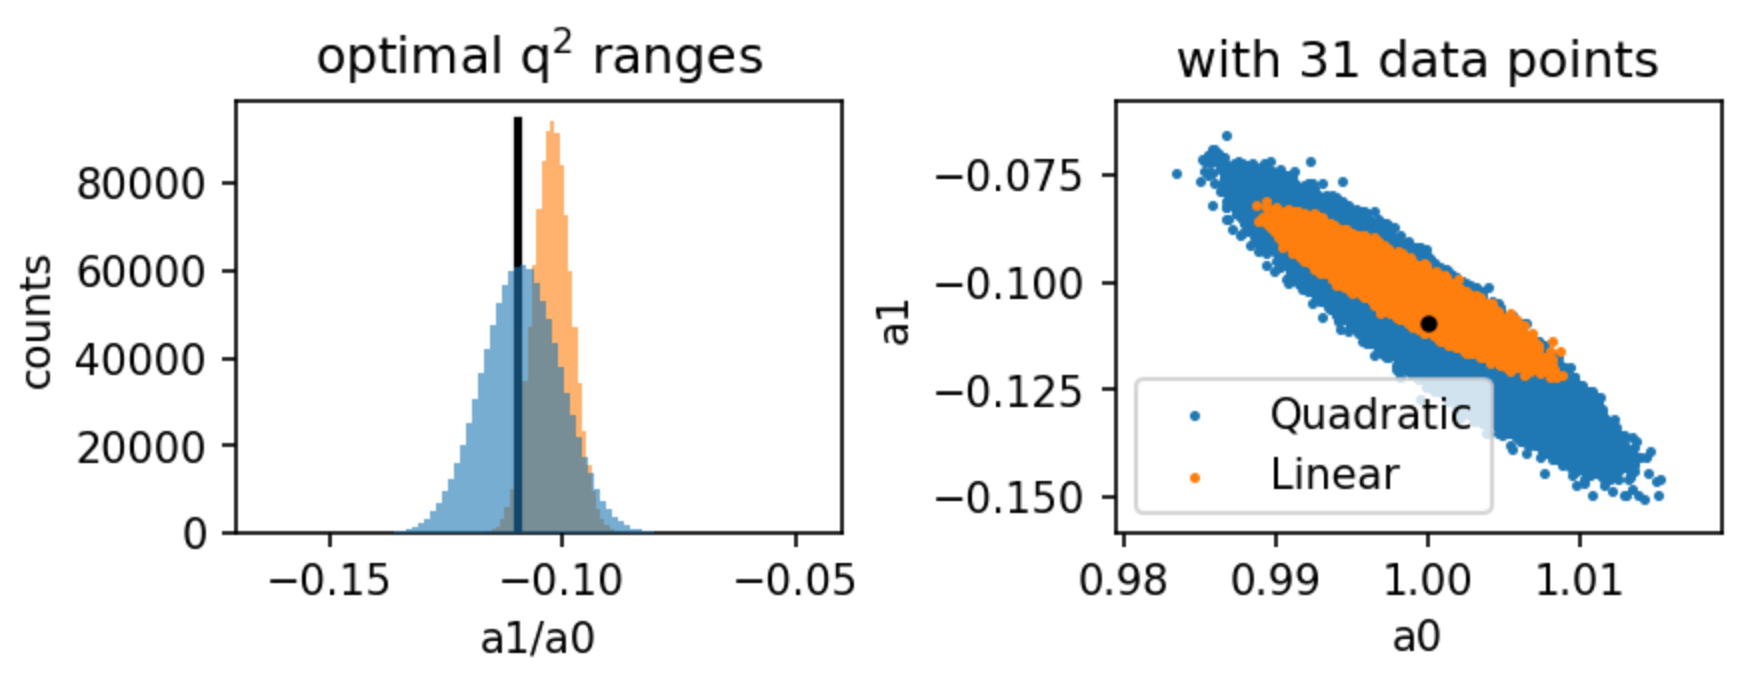
\includegraphics[width=\columnwidth]{Figure/zoptimized.png}
\caption{The result of a million simulations and fits of linear fits over the $Q^2$ range 
of0.1 -- 0.8~fm$^{-2}$ and quadratic fits over 0.1 -- 1.6~fm$^{-2}$, both with 31 uniformly spaced data points.    Using root mean
square error as the matrix, neither example is significantly better than the other for exacting the proton
radius.   This is analogous to a dart game between two equally skilled players: one who hits the bulls eye more 
often yet has a large spread (low bias but high variance), and another, equally skilled, player who has a 
tighter cluster of hits but an offset (high bias but low variance).}
\label{zoptimized}
\end{figure}

\section{The Best Predictive Model}

Selecting between a linear or quadratic regression of the more complex standard dipole function may seem 
a bit contrived, as one might naively think that just using the generating function itself would always yield the
best results.   To show that this is not in fact the case, 
we use the lowest $Q^2$ range, 0.1 -- 0.4 fm$^{-2}$, and replace the quadratic function 
with the generating function and a floating normalization term:
\begin{equation}
\label{eq:fitdipole}
f_{{\mathrm{Dipole Fit}}}(Q^2) =  n_0 ( 1 - b_1 Q^2 / 2)^{-2},
\end{equation}
where $n_0$ is the normalization factor and the radius is given by $\sqrt{-6 b_1}$.
Absolute random errors of 0.01, 0.005 and 0.003 with two different spacing of the data: 
0.05 fm$^{-2}$ spacing with 7 point and 0.005 fm$^{-2}$ 
spacing with 31 points.       
The results of fitting these pseudo data sets are shown in Table~\ref{simpleVSperfect}.    
While the linear fit always has the greater bias, the dipole fit has the greater 
variance; bringing the root mean square error very close for all the test cases.   
Hopefully, this example makes it clear that it is not just the number of points that matter, 
but the size of the uncertainties that is a critical parameter in model selection.

Of course for real data, nature hides the true generating function from us, so perhaps it is reassuring to know
that a reasonable approximation is able to reveal the underlying physics just as well as, if not better than, the
true function.   
To be clear, the lesson is not that one function is better than another; it is that for a given set of data,
the scientist is challenged to use the most appropriate model (either descriptive or predictive) for
the task at hand.   Further details on the general mathematics behind these example problems can be 
found in~\cite{Shmueli:2010}.    

\begin{table*}
\caption{For the lowest Q$^2$ interval, 0.1 to 0.4 fm$^{-2}$, we compare regressions with
a linear function (Eq.~\ref{Eq:linear}) to the dipole fit function (Eq.~\ref{eq:fitdipole}).   Keeping the range
fixed, a spacing of 0.05~fm$^{-2}$ (7 points) and 0.01~fm$^{-2}$ (31 points) was used
with various absolute random errors.  In several of these cases, the simple linear 
function provides a better predictive model then the true functional form and is never 
far from the true function.}
\begin{tabular}{cc|cccccc|cccccc} \hline
Data   & Random   & \multicolumn{6}{c|}{linear fit}                       & \multicolumn{6}{c}{dipole fit}            \\ 
Points & Error    & $a_0$ & Radius&a$_1/a_0$&  Bias  & Sigma &  RMSE  & $n_0$ & Radius& $b_1$  &  Bias  & Sigma &  RMSE   \\  \hline
7      & 0.01     & 0.9995& 0.7941& $-0.1051$& $-0.0046$& 0.0359& 0.0361 & 1.0001& 0.8108& $-0.1096$& $-0.0001$& 0.0378& 0.0378  \\ 
7      & 0.005    & 0.9995& 0.7946& $-0.1052$& $-0.0045$& 0.0174& 0.0180 & 1.0000& 0.8114& $-0.1097$& $-0.0000$& 0.0194& 0.0194  \\
7      & 0.003    & 0.9996& 0.7951& $-0.1054$& $-0.0043$& 0.0108& 0.0116 & 1.0000& 0.8114& $-0.1097$& $-0.0000$& 0.0114& 0.0114  \\ \hline
31     & 0.01     & 0.9996& 0.7944& $-0.1052$& $-0.0045$& 0.0186& 0.0191 & 1.0000& 0.8112& $-0.1097$& $-0.0000$& 0.0207& 0.0207  \\
31     & 0.005    & 0.9995& 0.7951& $-0.1054$& $-0.0043$& 0.0093& 0.0102 & 1.0000& 0.8113& $-0.1097$&  0.0000& 0.0103& 0.0103  \\
31     & 0.003    & 0.9995& 0.7953& $-0.1054$& $-0.0043$& 0.0056& 0.0070 & 1.0000& 0.8113& $-0.1097$&  0.0000& 0.0062& 0.0062   \\ \hline 
61     & 0.01     & 0.9995& 0.7949& $-0.1053$& $-0.0044$& 0.0135& 0.0142 & 1.0000& 0.8114& $-0.1097$&  0.0000& 0.0150& 0.0150  \\ 
61     & 0.005    & 0.9995& 0.7952& $-0.1054$& $-0.0043$& 0.0069& 0.0081 & 1.0000& 0.8114& $-0.1097$&  0.0000& 0.0073& 0.0073  \\ 
61     & 0.003    & 0.9995& 0.7952& $-0.1054$& $-0.0043$& 0.0040& 0.0059 & 1.0000& 0.8113& $-0.1097$&  0.0000& 0.0045& 0.0045  \\ \hline 
\end{tabular}
\label{simpleVSperfect}
\end{table*}

\begin{figure}[htb]
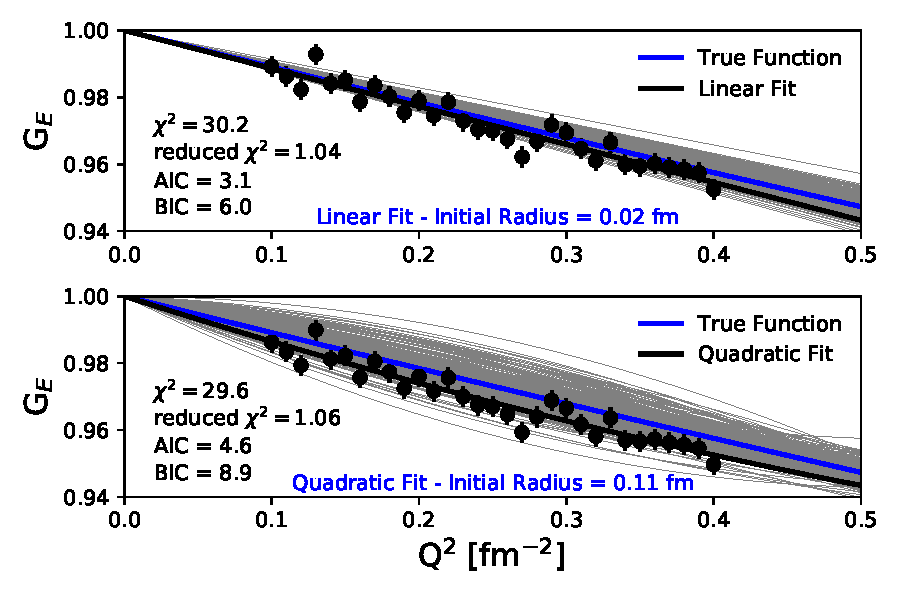
\includegraphics[width=\columnwidth]{Figure/linearVSquadratic-band.pdf}
\caption{Illustration of the effect of renormalizing data.  The
black points show one set of pseudo data, with absolute 0.3\% random point-to-point 
uncertainty and 0.01 fm$^{-2}$ spacing that have been renormalized
by applying the prior that $G_E(0)=1$.    While the prior is true, using an inappropriate model
can cause both the extracted radius and normalization to be dramatically shifted from the true
function.   
The grey bands were created by preforming of 250 simulations and are presented as
an animation in the supplemental material~\cite{Supplement}.}
\label{linearVSquadratic}
\end{figure}

\begin{figure}[htb]
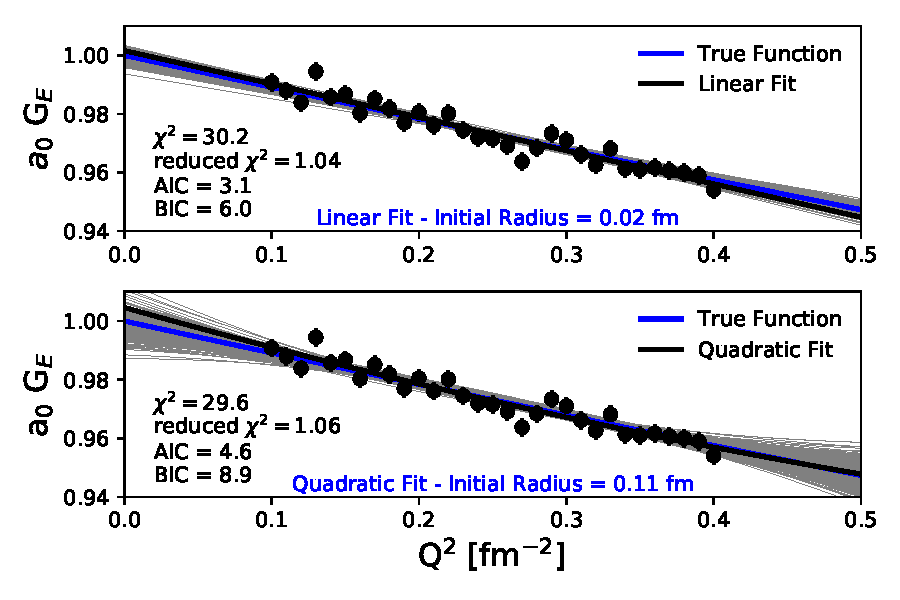
\includegraphics[width=\columnwidth]{Figure/frequentist-band.pdf}
\caption{Instead of applying the prior that $Q^2$ = 0 as done in Fig.~\ref{linearVSquadratic}, it is more natural to
just fit the data.  In fact, a frequentest would correctly simply check that the function reasonably points to one.
This version is also far more intuitive and more clearly shows how the quadratic function can bend as it extrapolates 
beyond the data.   
The grey bands were created using the same pseudo data as
as used in Fig.~\ref{linearVSquadratic}. 
and are presented as
an animation in the supplemental material~\cite{Supplement}. }
\end{figure}

To be clear, using an inappropriate model can lead to erroneous conclusions.
In Fig.~\ref{linearVSquadratic} we show an
example of one set of the pseudo data fit with a linear and quadratic where the prior that the
$G_E(0)=1$ has been applied (i.e. the data has been divided by the normalization term from the regression
so the function goes to the known limiting value at the origin).
Since here we know the function that generated the pseudo data, it is clear that the quadratic
fit has caused the data to be inappropriately shifted and will generate an unusually large radius, 
but in real life the true function is not known.
Note that we have left the initial normalization a constant since while the absolute normalization may be
unknown at the few percent level for a cross section measurement, its relative value for a given measurement
can be precisely monitored. 

\section{Model Selection}

While this classic Monte Carlo example problem is over 40 years old, it actually points to exactly the split in 
the current electron scattering proton radius extraction procedures.     The parsimonious modelers, who are 
focused solely on extracting a radius, have focused on the low $Q^2$ region accepting a slightly higher 
level of bias in exchange for low variance; on the other hand, those modelers who are interested in extracting more information 
about the proton (e.g. higher order moments) fit longer $Q^2$ ranges and have
focused on complex models which, while lower in bias, come at a cost of higher variance.  
It fact, the consequence of ever-increasing $Q^2$ ranges requiring increasing complexity have resulted in
an uncertainty in the extracted radius 
stuck at $\approx \unit[0.01]{fm}$ since L.~Hand~\textit{et al.}'s original fit in 1963~\cite{Hand:1963zz}.

Also, since we do not know the true model, one cannot in general calculate the RMSE. So, while Monte Carlo exercises 
like the one described herein are extremely useful for finding reasonable models to consider and understanding
expected uncertainties, the data must be used to select the appropriate model. 
For this one can rely on statistical modeling selection techniques such as an $F$-test for
nested models~\cite{Bevington:2003,James:2006,Sirca:2016} or the more general Akaike information criterion (AIC)~\cite{Akaike:1974} 
or Bayesian information criterion (BIC)~\cite{Schwarz:1978} 
to guide our selection of the most appropriate model to describe a given set of data.
These statistical criteria are calculated as follows: 
\begin{align}
\chi^2         & = \sum_{n=1}^{N}((\mathrm{data_i} - \mathrm{model}) / \sigma_i)^2, \\
reduced~\chi^2 & = \chi^2/ (N - N_{\mathrm{var}}),  \\
\mathrm{AIC}            & = N \log(\chi^2/N) + 2 N_{\mathrm{var}}, \\
\mathrm{BIC}            & = N \log(\chi^2/N) + \log(N) N_{\mathrm{var}},
\end{align}
where $N$ is the number of data points, $data_i$ and $\sigma_i$ are measured values and estimated uncertainties,
and $N_{\mathrm{var}}$ is the number of model parameters.
Further details about current model selection techniques can be found in~\cite{Ernst:2012}.

One should also always keep in mind that the input models in Monte Carlo simulations are always just an approximation
and one needs to be careful about drawing too strong inferences from the simulated results. 
For example, just because the linear model has a negative bias when compared to the standard dipole, 
does not imply that it has a negative bias with respect to all possible models.


\section{Real Data}

This bring us to the real data and the current proton radius extractions.   Many different functions have
been tried over the years from simple linear fits~\cite{Hand:1963zz,Murphy:1974zz} and continued fractions~\cite{Sick:2003gm} 
to high order polynomials~\cite{Bernauer:2013tpr,Lee:2015jqa} with and without constraints.   Since obtaining sub-percent
level cross sections is nearly impossible, a normalization parameter included to allow an entire set of data to shift
as was done in the Monte Carlo simulations.   Again, this just allows that the prior $G_E(0)=1$ can be applied.

The measured cross sections, $\sigma_{\mathrm{Meas}}$,  are related to the charge and electric form factors via 
\begin{equation}
\frac{\sigma_{\text{Meas}}}{\sigma_{\text{Mott}}} = \frac{n_0}{\varepsilon (1 + \frac{Q^2}{4M^2})} \left[\varepsilon G_E^2 (Q^2) + \frac{Q^2}{4M^2} G_M^2 (Q^2)\right],
\label{Eq:CrossSection}
\end{equation}
where $n_0$ is a normalization factor and the kinematic quantities $Q^2$ and $\varepsilon$ are given by
\begin{align}
Q^2 & = \frac{2M E^2 (1 - \cos{\theta})}{M + E (1 - \cos{\theta})}, \\
\varepsilon & = \left[1 + 2(1 + \frac{Q^2}{4M^2}  \tan^2{\frac{\theta}{2}})\right]^{-1}
\end{align}
where E is the incident electron beam energy, $M$~is the proton mass, $\theta$~is the measured electron scattering angle. 
The Mott cross section, $\sigma_{\text{Mott}}$, with the recoil factor included, is given by
\begin{equation}
\sigma_{\text{Mott}}  = \frac{\alpha^2}{4 E^2} \frac{\cos^2{(\theta / 2)}}{\sin^4{(\theta / 2)} ( 1 + \frac{E}{M} (1 - \cos{\theta}))}.
\end{equation}
%The known $\sigma_{\text{Mott}}$ term and the determined normalization can be divided out to report a renormalized reduced cross section
%\begin{equation}
%\sigma_{\text{Reduced}} = \frac{1}{n_0} \frac{ {\sigma_{\text{Meas}}}}{{\sigma_{\text{Mott}}}}.
%\label{Eq:Reduced}
%\end{equation}
From Eq.~\ref{Eq:CrossSection} is it clear that as $Q^2$ goes to zero and $\varepsilon$ goes to one (forward angle electron scattering), 
the terms which include the  magnetic form factor, $G_M$, are not very important which, is why this work has
focused on simply the charge form factor.

To illustrate the current tension between fit done with different models, Fig.~\ref{RealData} shows 
104 data points from one full subset from a modern electron scattering 
experiment~\footnote{Data from Mainz spectrometer B with a beam energy of 315 MeV with radiative and Coulomb corrections~\cite{Bernauer:2013tpr}.} 
that covers a range similar to the range studied herein.  By using a single set, only one floating normalization
parameter is required.
This one set of data covers a range similar to the 85 data point fits with 6 floating normalizations~\cite{Rosenfelder:1999cd,Hill:2010yb}.
Along with the data, four representative functions are shown using Eq.~\ref{Eq:CrossSection} with a standard magnetic form factor.
Two functions give radii that agree with the CODATA value for the proton
radius~\cite{Bernauer:2013tpr,Ye:2017gyb} and two that agree with the muonic Lamb shift measurements~\cite{Higinbotham:2015rja,Griffioen:2015hta}.
We note that this figure looks oddly similar to the pseudo data in Fig.~\ref{linearVSquadratic} but here the true function is unknown 
so it is not clear which curves are shifted with respect to the true reduced cross section values.

\begin{figure}
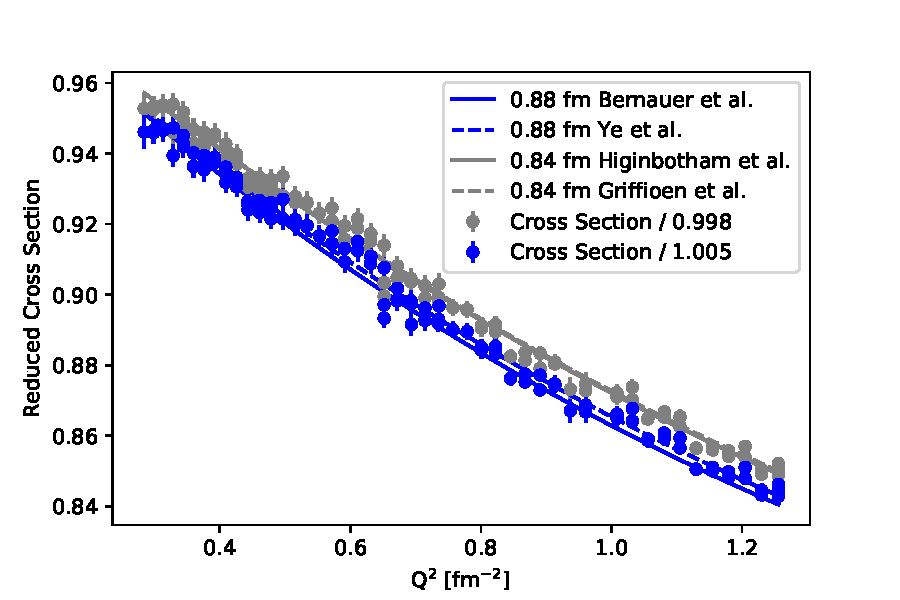
\includegraphics[width=\columnwidth]{Figure/RealData.pdf} 
\caption{Shown is one set of modern cross section data to illustrate the current tension between 
different models and the effect of the normalization parameter.   In electron scattering data, the
point-to-point uncertainties can be rather small, compared to the typical normalization uncertainty
of a few percent.   A standard magnetic
form factor has been used along with charge form factors from recent publications:  a bounded
13$^{th}$-order polynomial with a radius of 0.88~fm~\cite{Ye:2017gyb}, a unbounded 10$^{th}$-order polynomial with a radius of 0.88~fm~\cite{Bernauer:2013tpr}, 
a continued fraction with a radius of 0.84~fm~\cite{Griffioen:2015hta}, and a dipole function with a radius of 0.84~fm~\cite{Higinbotham:2015rja}. }
\label{RealData}
\end{figure}

Following the logic of this work, we try fitting the cross section data shown in Fig.~\ref{RealData} with  Eq.~\ref{Eq:CrossSection}, where
$G_E$ has been approximated by Eq.~\ref{Eq:linear} and Eq.~\ref{Eq:quadratic}, though with the normalization now subsumed in Eq.~\ref{Eq:CrossSection}.    
Additionally, we performed fits with the following two commonly used functions:
\begin{align}
f_{\mathrm{cubic}}(Q^2)   & = 1 + a_1 Q^2 + a_2 Q^4 + a_3 Q^6,  \\
f_{\mathrm{rational}}(Q^2) & = \frac{1+n_1 Q^2}{1+m_1 Q^2},
\end{align}
where the radius for the rational function is given by $\sqrt{-6 (n_1 - m_1)}$ and for the polynomials by $\sqrt{-6 a_1}$.
We note that the low order rational function ($n=m=1$) can easily be extended to give the expected asymptotic behavior
as $Q^2 \to \inf$ and that the more complex rational function ($n=1,m=1,2,3$) has been used in global fits~\cite{
Kelly:2004hm,
Puckett:2017flj,   
Gutsche:2017lyu}.

The fits were done first with a standard dipole magnetic form factor
and then repeated with the magnetic form factor from~\cite{Bernauer:2013tpr} and~\cite{Ye:2017gyb}.    
Using an $F$-test, AIC, or BIC for model selection all slightly prefer fits with Eq.~\ref{Eq:quadratic}.
It is important to note that the use of statistical criteria for model selection helps avoids confirmation bias,
though one could still be using an inappropriate function for the problem at hand. 
Uncertainties were determined by applying a statistical bootstrap to the data.   This is done
by repeatedly randomly sampling the true data with replacement to generate thousands of new sets of N points 
and refitting those new sets.   This allows one to get uncertainty distributions using the data itself and
avoids a number of assumptions that are required for $\chi^2$ uncertainty techniques 
to be valid~\cite{Efron:1979} and, unlike $\chi^2$ techniques, is also sensitive to over-fitting~\cite{Andrae:2010}.

\begin{table*}
\caption{Using four different magnetic form factor parameterizations, we extract the normalization
and radius using a linear, quadratic, cubic, and rational approximation for the $G_E$ function in 
Eq.~\ref{Eq:CrossSection}.
To avoid multiple floating multiple normalizations, the single set of 104 data points 
shown in Fig.~\ref{RealData} is used.
The parameter uncertainties were obtained using by performing statistical bootstraps of the data.
As seen during the Monte Carlo studies, the linear fit over this interval produces a small variance; 
but is clearly biased from the true 0.84--0.88~fm proton radius, whereas the quadratic with has a 
larger variance but gives less biased result.   The cubic fit function is over-fitting which is 
why it produces a huge variance.   The rational function is nearly as good as the quadratic through
produces a systematically larger radius though nicely in the range we expect.}
\begin{tabular}{cc|cccccl|cccccl}                                                  \hline \hline
\multicolumn{14}{l}{Standard Magnetic Form Factor}                                 \\ \hline
          &     & \multicolumn{6}{c}{without Coulomb correction}                 & \multicolumn{6}{|c}{with Coulomb correction} \\
$G_E$ Fit & df  & $\chi^2$ & reduced   & AIC    & BIC    & Norm      & Extrapolated & $\chi^2$ & reduced   & AIC    & BIC    & Norm      & Extrapolated      \\  
Function  &     &          & $\chi^2$  &        &        &           & Radius [fm]      &          & $\chi^2$  &        &        &           & Radius [fm]        \\ \hline
linear    & 102 & 162.6    & 1.594     & 50.47  & 55.74  & 0.988(1)  & 0.785(2)  & 167.2    & 1.639     & 53.35  & 58.64  & 0.985(1)  & 0.790(2)    \\
quadratic & 101 & 119.4    & 1.182     & 20.35  & 28.29  & 1.000(2)  & 0.852(10) & 119.0    & 1.178     & 20.00  & 27.93  & 0.998(2)  & 0.860(10)   \\
cubic     & 100 & 117.3    & 1.173     & 20.51  & 31.13  & 0.990(6)  & 0.785(57) & 117.1    & 1.171     & 20.33  & 30.90  & 0.990(6)  & 0.797(57)   \\    
rational  & 101 & 120.0    & 1.188     & 20.83  & 28.76  & 1.001(2)  & 0.860(10) & 119.6    & 1.184     & 20.50  & 58.64  & 0.999(2)  & 0.869(10)   \\ \hline \hline
\multicolumn{14}{l}{Kelly Magnetic Form Factor}                                   \\ \hline
          &     & \multicolumn{6}{c}{without Coulomb correction}                 & \multicolumn{6}{|c}{with Coulomb correction} \\
$G_E$ Fit & df  & $\chi^2$ & reduced   & AIC    & BIC    & Norm      & Extrapolated    & $\chi^2$ & reduced   & AIC    & BIC    & Norm      & Extrapolated     \\  
Function  &     &          & $\chi^2$  &        &        &           & Radius [fm]      &          & $\chi^2$  &        &        &           & Radius [fm]            \\ \hline
linear    & 102 & 168.1    & 1.648     & 53.95  & 59.24  & 0.986(1)  & 0.780(2)  & 173.0    & 1.669     & 53.35  & 58.64  & 0.985(1)  & 0.785(2)    \\
quadratic & 101 & 119.4    & 1.182     & 20.33  & 28.27  & 1.000(2)  & 0.852(10) & 119.0    & 1.178     & 20.00  & 27.91  & 0.998(2)  & 0.860(10)   \\
cubic     & 100 & 117.1    & 1.171     & 20.36  & 30.94  & 0.985(6)  & 0.598(57) & 116.9    & 1.169     & 20.14  & 30.72  & 0.983(6)  & 0.613(57)   \\    
rational  & 101 & 120.0    & 1.188     & 20.89  & 28.82  & 1.001(2)  & 0.861(10) & 119.6    & 1.188     & 20.87  & 28.80  & 1.001(2)  & 0.870(10)   \\ \hline \hline
\multicolumn{14}{l}{Bernauer Magnetic Form Factor}                                 \\ \hline
          &     & \multicolumn{6}{c}{without Coulomb correction}                 & \multicolumn{6}{|c}{with Coulomb correction} \\
$G_E$ Fit & df  & $\chi^2$ & reduced   & AIC    & BIC    & Norm      & Extrapolated    & $\chi^2$ & reduced   & AIC    & BIC    & Norm      & Extrapolated      \\  
Function  &     &          &$\chi^2$  &        &       &             & Radius [fm]      &          & $\chi^2$  &        &        &           & Radius [fm]            \\ \hline
linear    & 102 & 163.3    & 1.601     & 53.96  & 56.24 & 0.988(1)   & 0.786(2)  & 168.0    & 1.647     & 53.85  & 59.14  & 0.985(1)  & 0.791(2)    \\
quadratic & 101 & 119.5    & 1.183     & 20.44  & 28.37 & 1.000(2)   & 0.854(10) & 119.0    & 1.179     & 20.08  & 28.00  & 1.000(4)  & 0.862(10)    \\ 
cubic     & 100 & 117.3    & 1.173     & 20.52  & 31.13 & 0.992(6)   & 0.786(56) & 117.1    & 1.171     & 20.33  & 30.91  & 0.990(6)  & 0.797(56)    \\ 
rational  & 102 & 120.0    & 1.189     & 20.93  & 28.86 & 1.001(2)   & 0.871(13) & 119.7    & 1.185     & 20.60  & 28.54  & 0.999(2)  & 0.871(13)    \\ \hline \hline
\multicolumn{14}{l}{Ye Magnetic Form Factor}                                      \\ \hline
          &     & \multicolumn{6}{c}{without Coulomb correction}                 & \multicolumn{6}{|c}{with Coulomb correction} \\
$G_E$ Fit & df  & $\chi^2$ & reduced   & AIC    & BIC    & Norm      & Extrapolated    & $\chi^2$ & reduced   & AIC    & BIC    & Norm      & Extrapolated      \\  
Function  &     &          &$\chi^2$  &        &       &             & Radius [fm]      &          & $\chi^2$  &        &        &           & Radius [fm]    \\ \hline
linear    & 102 & 167.2    & 1.639    & 53.35  & 58.64 & 0.987(1)    & 0.781(2)  & 172.0    & 1.686     & 56.33  & 61.62  & 0.984(1)  & 0.786(2)    \\
quadratic & 101 & 119.4    & 1.182    & 20.33  & 28.26 & 1.000(2)    & 0.852(10) & 119.0    & 1.190     & 19.97  & 27.91  & 0.998(2)  & 0.860(10)    \\
cubic     & 100 & 117.3    & 1.173    & 20.55  & 31.12 & 0.992(6)    & 0.785(55) & 117.1    & 1.171     & 20.33  & 30.91  & 0.992(6)  & 0.797(55)    \\ 
rational  & 102 & 119.8    & 1.188    & 20.87  & 28.80 & 1.001(2)    & 0.860(14) & 119.6    & 1.184     & 20.54  & 28.48  & 0.999(2)  & 0.870(14)    \\ \hline \hline
\end{tabular}
\label{datatable}
\end{table*}
%# 
%#\begin{tabular}{ccccccc}                                                  \hline \hline
%#\multicolumn{6}{l}{Standard Magnetic Form Factor}                      \\ \hline
%#$G_E$ Fit & df  & reduced   & AIC    & BIC    & Norm      & Radius     \\  
%#Function  &     & $\chi^2$  &        &        &           & [fm]       \\ \hline
%#linear    & 102 & 1.639     & 53.35  & 58.64  & 0.985(1)  & 0.790(2)   \\
%#quadratic & 101 & 1.178     & 20.00  & 27.93  & 0.998(2)  & 0.860(10)  \\
%#cubic     & 100 & 1.171     & 20.33  & 30.90  & 0.990(6)  & 0.797(57)  \\    
%#rational  & 101 & 1.184     & 20.50  & 28.44  & 0.999(2)  & 0.869(10)  \\ \hline \hline
%#\multicolumn{6}{l}{Kelly Magnetic Form Factor}                         \\ \hline
%#$G_E$ Fit & df  & reduced   & AIC    & BIC    & Norm      & Radius     \\  
%#Function  &     & $\chi^2$  &        &        &           & [fm]       \\ \hline
%#linear    & 102 & 1.696     & 56.95  & 62.24  & 0.984(1)  & 0.785(2)   \\
%#quadratic & 101 & 1.178     & 20.00  & 27.91  & 0.998(2)  & 0.860(10)  \\
%#cubic     & 100 & 1.169     & 20.14  & 30.72  & 0.983(6)  & 0.613(57)  \\    
%#rational  & 101 & 1.188     & 20.87  & 28.80  & 1.001(2)  & 0.861(10)  \\ \hline \hline
%#\multicolumn{6}{l}{Bernauer Magnetic Form Factor}                      \\ \hline
%#$G_E$ Fit & df  &reduced   & AIC    & BIC   & Norm & Radius            \\  
%#Function  &     &$\chi^2$  &        &       &             & [fm]       \\ \hline
%#linear    & 102 & 1.647     & 53.85  & 59.14 & 0.985(1)   & 0.791(2)   \\
%#quadratic & 101 & 1.179     & 20.08  & 28.00 & 1.000(4)   & 0.862(10)  \\ 
%#cubic     & 100 & 1.171     & 20.33  & 30.91 & 0.990(6)   & 0.797(56)  \\ 
%#rational  & 102 & 1.185     & 20.60  & 28.54 & 0.999(2)   & 0.871(13)  \\ \hline \hline
%#\multicolumn{6}{l}{Ye Magnetic Form Factor}                            \\ \hline
%#$G_E$ Fit & df  & reduced  & AIC    & BIC   & Norm        & Radius     \\  
%#Function  &     &$\chi^2$  &        &       &             & [fm]       \\ \hline
%#linear    & 102 & 1.686    & 56.33  & 61.62 & 0.984(1)    & 0.786(2)   \\
%#quadratic & 101 & 1.190    & 19.97  & 27.91 & 0.998(2)    & 0.860(10)  \\
%#cubic     & 100 & 1.171    & 20.33  & 30.91 & 0.992(6)    & 0.797(55)  \\ 
%#rational  & 102 & 1.184    & 20.54  & 28.48 & 0.999(2)    & 0.870(14)  \\ \hline \hline
%#\end{tabular}
% Fits With The Normalization Fixed
%cubic-   & {\bf{1.011}}    & 4.143 & 12.077       & fixed-          & 0.832(5)     \\ 
%cubic+   & {\bf{1.103}}    &13.192 & 21.126       & fixed+          & 0.863(6)     \\ \hline \hline

It is of particular note that the quadratic fit is the same function over a similar range as found in the original 1976 work opting for
the quadratic fit~\cite{Borkowski:1975} though herein we 
use a single floating normalization instead of three and the point-to-point errors are smaller.   
It is perhaps distressing to note that published values of the 
radius extracted from electron scattering remained basically unchanged since the 1976 work~\cite{Borkowski:1975} while the 
functions used to make the extrapolation and obtained that same radius became increasingly complex and convoluted.
Oddly enough the standard dipole magnetic form factor quadratic fit has the lowest AIC and BIC values and gives a result consistent
with the muonic Lamb shift; though the rational function is nearly as good and is nearly exactly between the CODATA
and muonic Lamb shift values.    


\section{Graphs in Statistical Analysis}

Beyond simply checking statistic criteria, it is important to check the statistical analysis graphically~\cite{Anscombe:1973}.
The graphs help ensure that our underlying assumptions about the data are reasonably correct and help ensure that the results
aren't being overly influenced by a single point.   This is particularly important when doing $\chi^2$ minimizations where a
clear outlier can easily have an undue weight.    This is not to imply that one should simply remove an outlier, but it does
mean that one might wish to study the effect of fitting with and without the outlining point to clearly show its effect on 
the result.   The research can also review their notes to ensure that wasn't a mistake in the reporting of that point.

In top half of Fig.~\ref{residual}, the reported data is shown along with the quadratic fit:  best fit from Table~\ref{datatable} based
on AIC and BIC.   In the bottom half, the residual, a difference between the data and the model, is shown.     While these two plots
are perhaps the most common statistical analysis graph, they are not found in many highly cited proton radius papers and in fact some
paper  have no data quality plots at all (e.g.~\cite{Rosenfelder:1999cd}).
As the human eye will find patterns in statistical noise, the normal Q-Q plot is an important tool to check if in the fact the 
data is normally distributed~\cite{Wilk:1968}.   This is done in Fig.~\ref{normqq}, where the sorted residuals plotted against an normal distribution
and are shown to follow a normal distribution.   There are of course more formal statistical tests one can apply, but in general the
visualizations of the data can quickly reveal if there are any major problems.   In particular, with least squares fitting, one should
be mindful that a single outlier can skew the results.

\begin{figure}[htb]
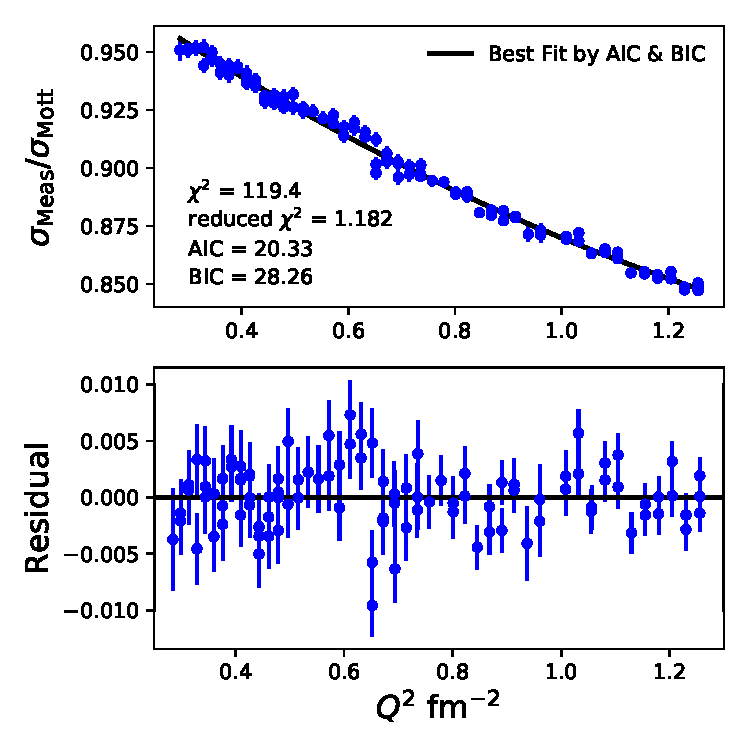
\includegraphics[width=\columnwidth]{Figure/NewVsOld.pdf}
\caption{The cross section data and the quadratic fit curve are shown in the upper plot and the residual, the difference between
the data and fit, are shown in the lower plot.    If an appropriate fit function was used, the Residuals should be randomly dispersed
dispersed around the horizontal axis.}
\label{residual}
\end{figure}

\begin{figure}[htb]
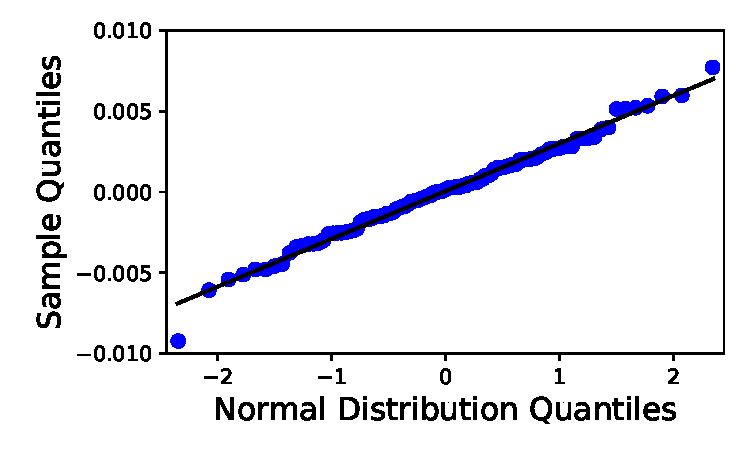
\includegraphics[width=\columnwidth]{Figure/NormQQ.pdf}
\caption{In order to check if the distribution of the residuals are plausibly normally distributed, one can make a normal
 quantile-quantile, Q-Q, plot.
This is done by sorting the residuals from lowest to highest and plotting the ordered residuals against a theoretical 
normal distribution.   The resulting plot is a beautiful example of normally distributed residuals.}
\label{normqq}
\end{figure}

\section{Lowest $Q^2$ Data} 

While the set of Mainz data studied above had a range similar to the large range of classic Monte Carlo studies, it wasn't
the lowest $Q^2$ set of data.   The lowest set comes from a run with 180 MeV 
and covers a range from 0.090 to 0.330 fm$^{-2}$.   This range is particularly integraing as it has been shown to be
low enough that even a linear regress should be able to extract the radius; though instead of just relying on the Monte
Carlo study to make that choice, we once again systematical look at the data with various function and variance choices
for the magnetic form factor in Table~\ref{lowestdatatable}.

\begin{table*}
\caption{Using four different magnetic form factor parameterizations, we extract the normalization
and radius using a linear, quadratic, cubic, and rational approximation for the $G_E$ function in 
Eq.~\ref{Eq:CrossSection}.
To avoid multiple floating multiple normalizations, the single set of 106 data points 
shown in Fig.~\ref{RealData} is used.
The parameter uncertainties were obtained using by performing statistical bootstraps of the data.
As seen during the Monte Carlo studies, the linear fit over this interval produces a small variance; 
but is clearly biased from the true 0.84--0.88~fm proton radius, whereas the quadratic with has a 
larger variance but gives less biased result.   The cubic fit function is over-fitting which is 
why it produces a huge variance.   The rational function is nearly as good as the quadratic through
produces a systematically larger radius though nicely in the range we expect.}
\begin{tabular}{cc|cccccl|cccccl}                                                  \hline \hline
\multicolumn{14}{l}{Standard Magnetic Form Factor}                                 \\ \hline
          &     & \multicolumn{6}{c}{without Coulomb correction}                 & \multicolumn{6}{|c}{with Coulomb correction} \\
$G_E$ Fit & df  & $\chi^2$ & reduced   & AIC    & BIC    & Norm      & Extrapolated& $\chi^2$ & reduced   & AIC    & BIC    & Norm      & Extrapolated    \\  
Function  &     &          & $\chi^2$  &        &        &           & Radius [fm]      &          & $\chi^2$  &        &        &           & Radius [fm]        \\ \hline
linear    & 104 &  69.2    & 0.666     &$-41.14$&$-35.81$& 1.000(1)  & 0.826(8)  &  69.6    & 0.670     &$-40.53$&$-35.21$& 0.997(1)  & 0.842(8)    \\
quadratic & 103 &  67.0    & 0.651     &$-42.58$&$-34.59$& 1.006(3)  & 0.923(50) &  66.9    & 0.649     &$-42.80$&$-34.81$& 1.004(3)  & 0.948(50)   \\
cubic     & 102 &  66.3    & 0.650     &$-41.79$&$-31.13$& 0.996(6)  & 0.598(nan)&  66.2    & 0.649     &$-41.95$&$-31.30$& 0.994(6)  & 0.645(nan)   \\    
rational  & 103 &  63.8    & 0.632     &$-43.77$&$-30.46$& 0.934(3)  & 0.936(55) &  67.0    & 0.650     &$-42.63$&$-34.64$& 1.004(3)  & 0.964(55)   \\ \hline \hline
\multicolumn{14}{l}{Kelly Magnetic Form Factor}                                   \\ \hline
          &     & \multicolumn{6}{c}{without Coulomb correction}                 & \multicolumn{6}{|c}{with Coulomb correction} \\
$G_E$ Fit & df  & $\chi^2$ & reduced   & AIC    & BIC    & Norm      & Extrapolated    & $\chi^2$ & reduced   & AIC    & BIC    & Norm      & Extrapolted      \\  
Function  &     &          & $\chi^2$  &        &        &           & Radius [fm]      &          & $\chi^2$  &        &        &           & Radius [fm]            \\ \hline
linear    & 104 &  69.3    & 0.666     &$-41.03$&$-35.70$& 1.000(1)  & 0.824(8)  &  69.7    & 0.670     &$-40.41$&$-35.08$& 0.998(1)  & 0.840(8)    \\
quadratic & 103 &  67.0    & 0.651     &$-42.58$&$-34.59$& 1.000(2)  & 0.923(50) &  66.9    & 0.649     &$-42.80$&$-34.81$& 1.004(2)  & 0.948(50)   \\
cubic     & 102 &  66.2    & 0.649     &$-41.86$&$-31.21$& 0.995(6)  & 0.525(nan)&  66.1    & 0.648     &$-42.03$&$-31.38$& 0.993(6)  & 0.578(nan)   \\    
rational  & 103 &  67.1    & 0.652     &$-42.43$&$-34.44$& 1.006(3)  & 0.937(55) &  67.0    & 0.651     &$-42.62$&$-34.63$& 1.005(3)  & 0.965(55)   \\ \hline \hline
\multicolumn{14}{l}{Bernauer Magnetic Form Factor}                                 \\ \hline
          &     & \multicolumn{6}{c}{without Coulomb correction}                 & \multicolumn{6}{|c}{with Coulomb correction} \\
$G_E$ Fit & df  & $\chi^2$ & reduced   & AIC    & BIC    & Norm      & Extrapolated  & $\chi^2$ & reduced   & AIC    & BIC    & Norm      & Extrapolated      \\  
Function  &     &          &$\chi^2$   &        &        &           & Radius [fm]   &          & $\chi^2$  &        &        &           & Radius [fm]            \\ \hline
linear    & 104 &  69.2    & 0.665     &$-41.19$&$-35.87$& 1.001(1)  & 0.826(8)  &  69.9    & 0.669     &$-40.59$&$-35.26$& 0.984(1)  & 0.842(8)    \\
quadratic & 103 &  67.0    & 0.651     &$-42.58$&$-34.59$& 1.006(2)  & 0.923(50) &  66.9    & 0.649     &$-42.80$&$-34.81$& 1.004(4)  & 0.948(50)    \\ 
cubic     & 102 &  66.2    & 0.650     &$-41.79$&$-31.13$& 0.996(6)  & 0.598(nan)&  66.2    & 0.649     &$-41.95$&$-31.30$& 0.994(6)  & 0.645(nan)    \\ 
rational  & 103 &  67.1    & 0.652     &$-42.44$&$-34.44$& 1.007(3)  & 0.936(55) &  67.0    & 0.650     &$-42.63$&$-34.64$& 0.999(3)  & 0.964(55)    \\ \hline \hline
\multicolumn{14}{l}{Ye Magnetic Form Factor}                                      \\ \hline
          &     & \multicolumn{6}{c}{without Coulomb correction}                 & \multicolumn{6}{|c}{with Coulomb correction} \\
$G_E$ Fit & df  & $\chi^2$ & reduced   & AIC    & BIC    & Norm      & Extrapolated & $\chi^2$ & reduced   & AIC    & BIC    & Norm      & Extrapolated      \\  
Function  &     &          &$\chi^2$   &        &        &           & Radius [fm]      &          & $\chi^2$  &        &        &       & Radius [fm]     \\ \hline
linear    & 104 &  69.3    & 0.666     &$-41.04$&$-35.71$& 1.000(1)  & 0.824(8)  &  69.7    & 0.670     &$-40.42$&$-35.09$& 0.998(1)  & 0.841(8)    \\
quadratic & 103 &  67.0    & 0.651     &$-42.58$&$-34.59$& 1.006(2)  & 0.923(50) &  66.9    & 0.649     &$-42.80$&$-34.81$& 1.004(2)  & 0.948(50)    \\
cubic     & 102 &  66.3    & 0.650     &$-41.79$&$-31.13$& 0.996(6)  & 0.598(nan)&  66.2    & 0.649     &$-41.95$&$-31.30$& 0.994(6)  & 0.645(nan)    \\ 
rational  & 103 &  67.1    & 0.652     &$-42.43$&$-34.44$& 1.007(3)  & 0.936(55) &  67.0    & 0.651     &$-42.62$&$-34.63$& 1.005(3)  & 0.964(55)    \\ \hline \hline
\end{tabular}
\label{lowestdatatable}
\end{table*}

\begin{figure}[htb]
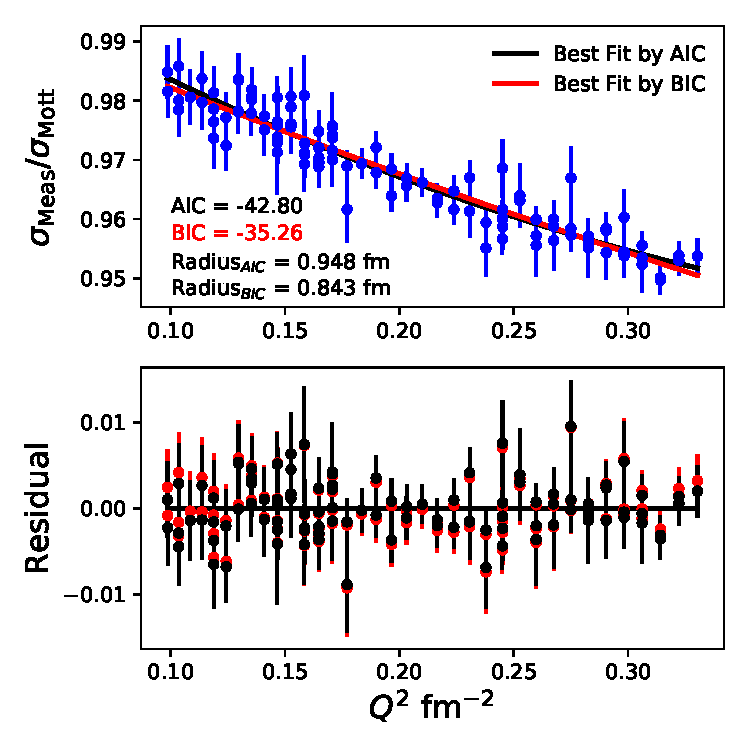
\includegraphics[width=\columnwidth]{Figure/BestLow.pdf}
\caption{The cross section data and the quadratic fit curve are shown in the upper plot and the residual, the difference between
the data and fit, are shown in the lower plot.}
\label{residual}
\end{figure}

\begin{figure}[htb]
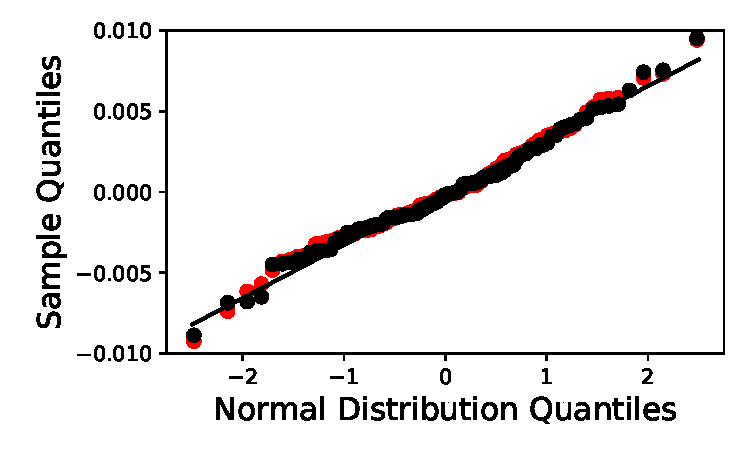
\includegraphics[width=\columnwidth]{Figure/LowNormQQ.pdf}
\caption{
The low $Q^2$ data quite as normally distributed residuals though still reasonable close to what one would expect.}
\label{normqq}
\end{figure}

It is important to note while these fits look beautiful, the extraction of the radius is an
extrapolation our belief that we can reasonably expect our function to extrapolate is based
on the Monte Carlo study at the beginning of the paper.    And while it is certainly reasonable
to assume the the charge form factor will smoothly continue to $Q^2$ = 0,
nature will do as it wishes and new data covering the 0 to 0.1~fm$^{-2}$ range is 
certainly desirable to ensure that our anzats is in fact correct~\cite{Gasparian:2014rna,
Peng:2016szv, Mihovilovic:2016rkr}.   
Also, strictly speaking, the
uncertainties from the regressions are only valid over the range of the data, so again our 
belief that we are obtaining reasonable uncertainties links back to the Monte Carlo study of the
radius extraction using different functions and the relatively short distance of the extrapolation.

As has been shown clearly by theory calculations
such as Alarcon and Weiss~\cite{}, the moments of the generating function are far too complex to be constrained
by fitting.  Also, as pointed out on page XXX of \cite{}, moments do not uniquely define functions, so the best
we can do for the higher order terms is determine the shape of the data and then compare with theory.

Another problem is the human-in-the-loop factor~\cite{Daee:2018:UMA:3172944.3172989}.   It is clear 
reading through the literature, that often the people fitting the data are the
same ones as those making the data selection decisions.
It is worth noting, that the PRad collaboration has come up with their model selection techniques
prior to looking at the real data~\cite{Yan:2018bez}.

\section{Higher Order Terms}

For higher order terms, we turn to theory instead of continuing with polynomial fitting. 

\section{Summary}

This work was in not meant to be an exhaustive study of the world electron scattering data; but 
instead explore the concept of bias-variance trade-off as it relates to the extraction of the proton 
radius from electron scattering data and show that parsimonious modeling can in fact have better 
predictive power then a more baroque models in certain situations.   Thus the model selection techniques
presented herein provide a rigorous method of selecting the most appropriate model to describe a given
set a data.

Also, using a set of electron scattering data with its single normalization parameter, we 
illustrated these model selection techniques as well as 
some key statistical analysis plots that should be produced in order to ensure a reasonable fit.   
While just a single realization of the data, this example serves to illustrate the current tension 
between electron scattering fitters who are actually not just differing about the radius of the
proton but also on the absolute normalization of the electron scattering data.
It is interesting to note that while the Frequentest
seeks the best model to describe the data, a Bayesian would likely look at the collection of results as  
subset of the possible ways the data can be normalized and the radius extracted (e.g. Gaussian process 
regression~\cite{Rasmussen:2005}).    

For the specific example of electron scattering, we have revisited a classic Monte Carlo study and shown
the common practice of simply concluding that one should reject models with a bias is incorrect
as it the assumption that you can add more regression parameters simply because you have more data.  
These idea are not constrained to the physical sciences, but also extends 
to quantitative analysis~\cite{Brighton:2015} and it is at the heart of statistical 
learning~\cite{Hastie:2009}.
This important concept of the power of parsimonious modeling was nicely 
summarized by the renowned statistician George Box: 
``Since all models are wrong the scientist cannot obtain a `correct' one
by excessive elaboration.  On the contrary, following William of Occam, 
[the scientist] should seek an economical description of natural phenomena. 
Just as the ability to devise simple but evocative models is the signature of the
great scientist so over-elaboration and over-parameterization is often
the mark of mediocrity.''~\cite{Box76}


\begin{acknowledgments}
The regressions done in this work were done in Python making use of the
outstanding LMFIT package~\cite{Newville:2014} to interface with SciPy
libraries~\cite{Jones:2001}.  Non-linear regressions were done using the
Levenberg–Marquardt method~\cite{Marquardt:1963}.
This work was supported by the U.S.  Department of Energy contract DE-AC05-06OR23177
under which Jefferson Science Associates operates the Thomas Jefferson National 
Accelerator Facility and contract DE-FG02-03ER4123 at Duke University.
\end{acknowledgments}


\appendix*
\section{Anscombe Quartet}

As nuclear physicists tend to use reduced $\chi^2$ instead of R$^2$, we have taken the 1973 example
problem of F. J. Anscombe~\cite{Anscombe:1973} and added uncertainties to the data points.

\begin{table}[htb]
\caption{Four data sets of (x,y,dy) values.}
\begin{tabular}{rccccccc}
\multicolumn{1}{l}{Data set}    & 1-3  & 1    & 2    & 3    & 4   & 4    & 1-5   \\
\multicolumn{1}{l}{Variable}    & x    & y    & y    & y    & x   & y    & dy    \\  
            &      &      &      &      &     &      &       \\
Obs. no. 1: & 10.0 & 8.04 & 9.14 & 7.46 & 8.0 & 6.58 & 1.235 \\ 
         2:   &  8.0 & 6.95 & 8.14 & 6.77 & 8.0 & 5.76 & 1.235 \\
         3:   & 13.0 & 7.58 & 8.74 &12.74 & 8.0 & 7.71 & 1.235 \\
         4:   &  9.0 & 8.81 & 8.77 & 7.11 & 8.0 & 8.84 & 1.235 \\
         5:   & 11.0 & 8.33 & 9.26 & 7.81 & 8.0 & 8.47 & 1.235 \\
         6:   & 14.0 & 9.96 & 8.10 & 8.84 & 8.0 & 7.04 & 1.235 \\
         7:   &  6.0 & 7.24 & 6.13 & 6.08 & 8.0 & 5.25 & 1.235 \\
         8:   &  4.0 & 4.26 & 3.10 & 5.39 &19.0 &12.50 & 1.235 \\
         9:   & 12.0 &10.84 & 9.13 & 8.15 & 8.0 & 5.56 & 1.235 \\
       10:    &  7.0 & 4.82 & 7.26 & 6.42 & 8.0 & 7.91 & 1.235 \\
       11:    &  5.0 & 5.68 & 4.74 & 5.73 & 8.0 & 6.89 & 1.235 \\ 
            &      &      &      &      &     &      &       \\ \hline
\end{tabular}
\end{table}

These four sets of (x,y,dy) values give to three significant figures that exact
same statisiical quanites: mean, variance, $\chi^2$, reduced $\chi^2$, etc.
So if one fails to make graphical checks, one can be completely fooled as is 
easily seen by graphing the data~\ref{SameChi2}.

\begin{figure}
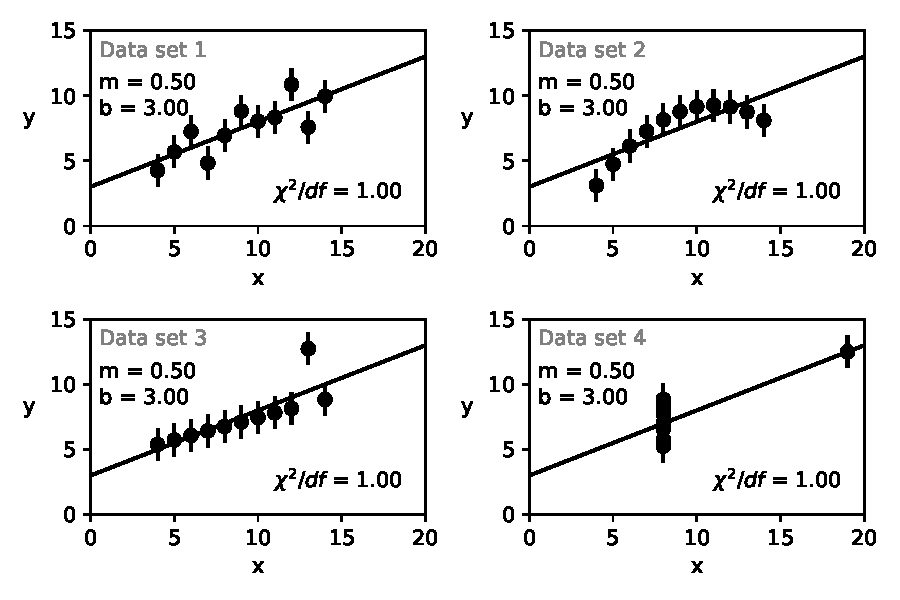
\includegraphics[width=\columnwidth]{Figure/SameChi2.pdf}
\caption{Four sets}
\label{SameChi2}
\end{figure}









\bibliography{elastic}

\end{document}
